Consider the polynomials $\phi_1(x) = 1$, $\phi_2(x) = x$, 
and $\phi_3(x) = 3x^2-1$, which form a basis for the set
of all quadratic polynomials.  These polynomials are 
orthogonal in $C[-1,1]$ with the usual inner product
\[ \ip{u,v} = \int_{-1}^1 u(x)v(x)\, dx.\]
(You do not need to prove this.) In the parts below,
``best approximation'' is defined with respect to this
inner product, and the norm it induces.

Let $f(x) = \cos(\pi x)$.
\begin{enumerate}
\item Construct the best approximation
           $f_1(x) = c_1 \phi_1(x)$
      to $f(x)$ from ${\rm span}\{\phi_1\}$ \\
      (i.e., determine $c_1$ to minimize $\norm{f - f_1}$ in $C[-1,1]$).
\vspace*{1em}
\item Construct the best approximation
           $f_2(x) = c_1 \phi_1(x) + c_2 \phi_2(x)$
      to $f(x)$ from ${\rm span}\{\phi_1, \phi_2\}$.
\vspace*{1em}
\item Construct the best approximation
           $f_3(x) = c_1 \phi_1(x) + c_2 \phi_2(x) + c_3 \phi_3(x)$
      to $f(x)$ from ${\rm span}\{\phi_1, \phi_2, \phi_3\}$.
\vspace*{-.25em}
\item  Produce a plot that superimposes your best approximation from parts~(a),
       (b), and (c) on top of a plot of $f(x)$.
\end{enumerate}

%%%%%%%%%%%%%%%%%%%%%%%%%%%%%%%%%%%%%%%%%%%%%%%%%%%%%%%%%%%%%%%%%%%%%%%%%%%%%%%%

\ifthenelse{\boolean{showsols}}{\begin{solution}

\begin{enumerate}
\item The best approximation to $f(x) = \cos(\pi x)$ from ${\rm span}\{\phi_1\}$ 
      on $[0,1]$ in the usual inner product is
       \[ f_1(x) = {(f,\phi_1) \over (\phi_1, \phi_1)} \phi_1(x).\]
      We compute
      \begin{eqnarray*} 
          \ip{\phi_1,\phi_1} &=& \int_{-1}^1 1^2\,dx = 2 \\[0.5em]
          \ip{f,\phi_1} &=& \int_{-1}^1 1\cdot\cos(\pi x)\,dx = 0,\\[0.5em]
      \end{eqnarray*} 
      and hence the best approximation is trivial:
       \[ f_1(x) = 0 \cdot \phi_1(x) = 0.\]
\item To compute the best approximation from ${\rm span}\{\phi_1, \phi_2\}$, we 
      can follow two approaches.  If we notice that $\phi_1$ and $\phi_2$ are
      orthogonal, i.e., $(\phi_1, \phi_2) = 0$, we can directly compute the
      best approximation as the sum of the best approximation from each 
      of the one dimensional subspaces:
       \[ f_2(x) = {(f,\phi_1) \over (\phi_1, \phi_1)} \phi_1(x)
                  + {(f,\phi_2) \over (\phi_2, \phi_2)} \phi_2(x).\]
      Noting, in addition to the quantities from part~(a), that
      \begin{eqnarray*}
         \ip{\phi_2,\phi_2} &=& \int_{-1}^1 x^2\,dx = 2/3 \\[0.5em]
         \ip{f,\phi_2} &=& \int_{-1}^1 x\cdot\cos(\pi x)\,dx = 0, 
      \end{eqnarray*}
      we again find the trivial approximation:
       \[ f_2(x) = 0\cdot  \phi_1(x) + 0\cdot \phi_2(x) = 0.\]
  
      Alternatively, we could have arrived at this approximation via the
      linear system
\[ \bmatrix{ \ip{\phi_1,\phi_1} & \ip{\phi_1,\phi_2} \cr
             \ip{\phi_2,\phi_1} & \ip{\phi_2,\phi_2} }
   \bmatrix{c_1 \cr c_2 } 
  = \bmatrix{ \ip{f,\phi_1} \cr 
              \ip{f,\phi_2}}.\]
       Using $(\phi_1,\phi_2) = (\phi_2,\phi_1) = 0$ gives the same trivial result
       as above. 
\item 
We can find the coefficients of $f_3(x) = c_1 \phi_1(x) + c_2 \phi_2(x) + c_3 \phi_3(x)$
by noting that all three basis functions are orthogonal, 
 \[ (\phi_1,\phi_2) = (\phi_1,\phi_3) = (\phi_2,\phi_3) = 0,\]
and thus constructing
       \[ f_3(x) = {(f,\phi_1) \over (\phi_1, \phi_1)} \phi_1(x)
                  + {(f,\phi_2) \over (\phi_2, \phi_2)} \phi_2(x)
                  + {(f,\phi_3) \over (\phi_3, \phi_3)} \phi_3(x).\]
Toward this end, compute
\begin{eqnarray*}
  \ip{\phi_3,\phi_3} &=& \int_{-1}^1 (3x^2-1)^2\,dx = 8/5 \\[0.5em]
  \ip{\phi_3,f} &=& \int_{-1}^1 (3x^2-1)\cdot\cos(\pi x)\,dx = -12/\pi^2,
\end{eqnarray*}
thus giving
       \[ f_3(x) = 0\cdot  \phi_1(x) + 0\cdot \phi_2(x) + {-12/\pi^2 \over 8/5} \phi_3(x) = {-15\over 2 \pi^2} (3x^2-1) .\]
Alternatively we can solve the linear system,
\[ \bmatrix{ \ip{\phi_1,\phi_1} & \ip{\phi_1,\phi_2} & \ip{\phi_1,\phi_3} \cr
             \ip{\phi_2,\phi_1} & \ip{\phi_2,\phi_2} & \ip{\phi_2,\phi_3} \cr
             \ip{\phi_3,\phi_1} & \ip{\phi_3,\phi_2} & \ip{\phi_3,\phi_3}}
   \bmatrix{c_1 \cr c_2 \cr c_3}
  = \bmatrix{ \ip{\phi_1, f} \cr 
              \ip{\phi_2, f} \cr
              \ip{\phi_3, f}} \]
whose coefficients have already been computed, except for
\begin{eqnarray*}
  \ip{\phi_3,\phi_1} = \ip{\phi_1, \phi_3} 
                     &=& \int_{-1}^1 1 (3x^2-1)\,dx = 0 \\[0.5em]
  \ip{\phi_3,\phi_2} = \ip{\phi_3, \phi_2} 
                     &=& \int_{-1}^1  x (3x^2-1)\,dx = 0,
\end{eqnarray*}
i.e., the basis vectors $\phi_1$, $\phi_2$, and $\phi_3$ are orthogonal.
Since the matrix is diagonal, the coefficients $c_1$, $c_2$, and $c_3$ are simple to find:
\begin{eqnarray*}
    c_1 &=& \ip{\phi_1,f}/\ip{\phi_1,\phi_1} = 0 \\[0.5em]
    c_2 &=& \ip{\phi_2,f}/\ip{\phi_2,\phi_2} = 0 \\[0.5em]
    c_3 &=& \ip{\phi_3,f}/\ip{\phi_3,\phi_3} = -15/(2\pi^2).
\end{eqnarray*}
Thus the best approximation to $\cos(\pi x)$ from the quadratic polynomials is
\[ f_3(x) = {15\over 2\pi^2} (1-3x^2).\]

\item The following plot compares best approximations to $f(x)$.
Note that $f_2$ obscures $f_1$.

[\textbf{GRADERS}: the code for making such a plot is so basic that students
do not need to include it.  If they omitted the code, please do not subtract
points here.]

\begin{center} 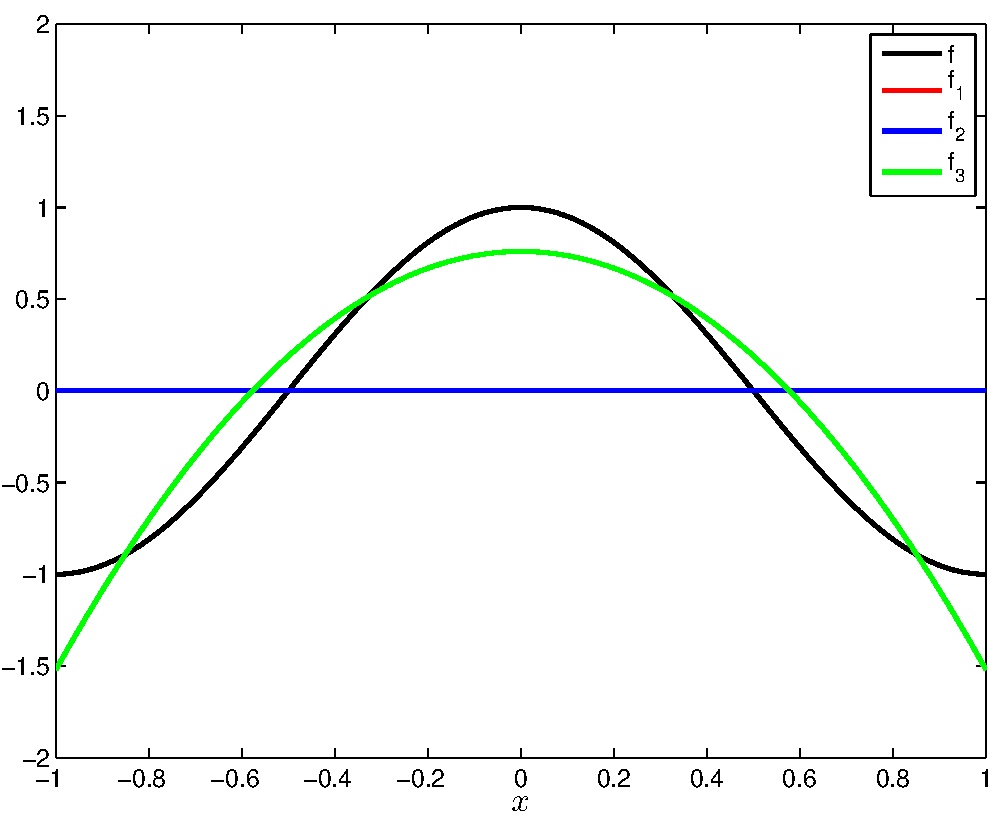
\includegraphics[scale=0.5]{legendre} \end{center}

\end{enumerate}
A more interesting series of approximations follows for $f(x) = e^x$, as 
seen in the following figure.
\begin{center} 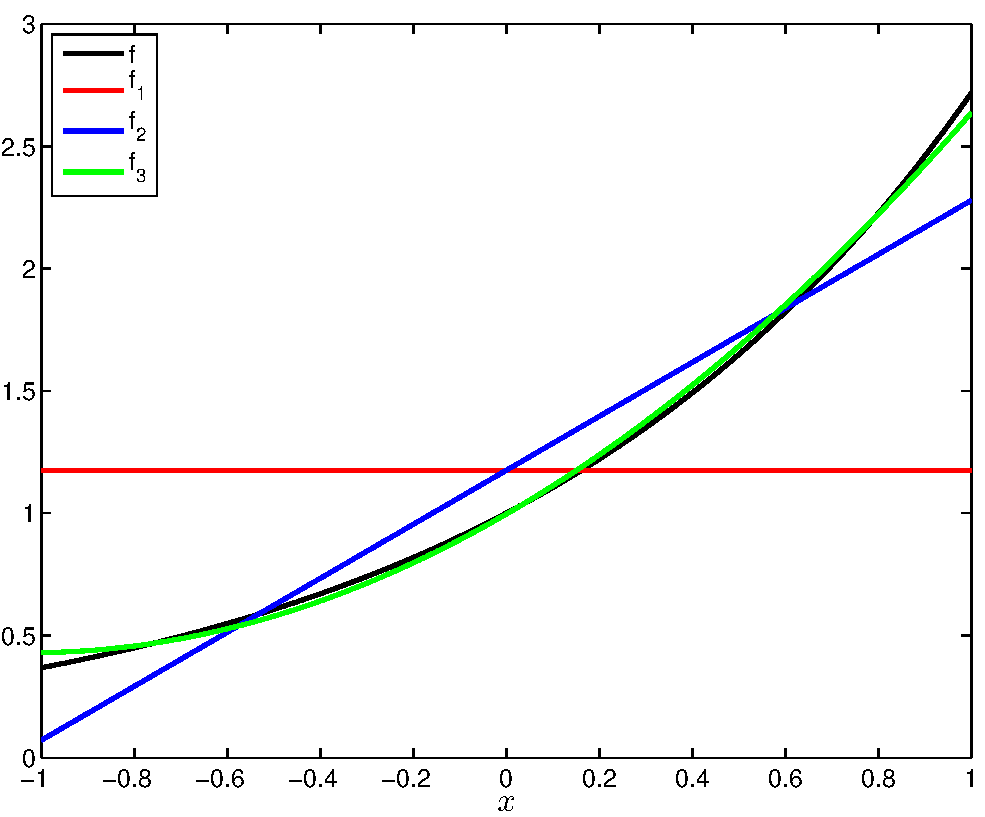
\includegraphics[scale=0.5]{legendre_exp} \end{center}

\end{solution}}{}

